% !TEX root = demoReport.tex
\section*{Problem 2: Stochastic Local Search (SLS)}

%\todo{
%  %% delete this paragraph, including its footnote:
%  The \emph{investment design problem} is about finding a matrix of
%  $v$~rows and $b$~columns of~$0$-$1$ integer values, such that each
%  row sums up to~$r$, with $v \geq 2$ and $b \geq r \geq 1$, and the
%  largest dot product between all pairs of rows is minimised.
%  % 
%  Equivalently, one has to find~$v$ subsets of size~$r$ within a given
%  set of $b$~elements, such that the largest intersection of any two
%  of the $v$~sets has minimal size.
%  % 
%  An instance of the problem is parametrised by a
%  triple~$\Tuple{v,b,r}$.\footnote{\todo{Your report need not contain
%      an explanation of the problem to be solved: you can assume the
%      reader has read th e problem statement in the assignment
%      instructions.  We just repeat it here for self-sufficiency of
%      this document.}}
%  
%  %% delete this paragraph:
%  This is an abstract description of a problem that appears in
%  finance: see Figure~\ref{fig:wallStreet}.  In a typical investment
%  design in finance, we have $4 \leq v \leq 25$ and
%  $250 \leq b \leq 500$, with $r \approx 100$.
%
%  %% delete this figure:
%  \begin{figure}[b]  % make it float to the bottom of a page
%    \centering
%    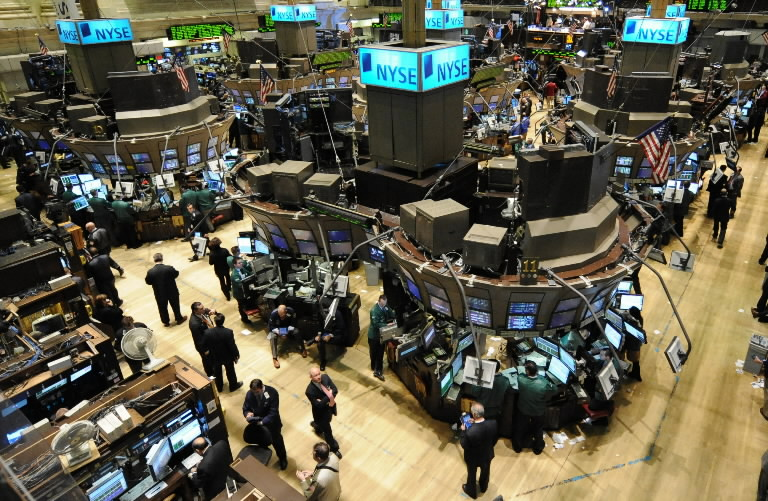
\includegraphics[height=5cm]{wallStreet}
%    \caption{\todo{Wall Street (\copyright\ www.forbes.com, 2014)}}
%    \label{fig:wallStreet}
%  \end{figure}
%  
%  %% delete this paragraph, if you want:
  A lower bound on the number~$\lambda$ of shared elements of any
  pair among $v$~subsets of size~$r$ drawn from a given set of
  $b$~elements is given in~\cite{ASTRA:AOC}:
  \begin{equation}\label{eq:lb}
  \text{lb}(\lambda) = 
    \Ceiling{
      \frac{\Ceiling{\frac{rv}{b}}^{2} ((rv) \bmod b)  +
        \Floor{\frac{rv}{b}}^{2} (b - ((rv) \bmod b)) - rv}
      {v(v-1)}
    }
  \end{equation}
%  
%}

\paragraph{Task~a: SLS Algorithm.}
\begin{enumerate}
\item Representation. 
The current state of the local search is given by a $v \times b$ matrix, where each row $v$ is a binary array of length $b$ where there are always $r$ elements that are $1$. 
%\todo{Describe how to represent the problem:
%  what are the variables, their meanings, their constraints, and the
%  objective function?}

  
\item Initial Assignment. It is made by randomly generating $v$ binary arrays where $r$ ones are randomly positioned. %\todo{Describe an algorithm for generating
%  (fast) a randomised initial assignment.}
\item Move. Each move we make is a switch in one row, making a permutation of a zero element with a one element. 
%. With a probability of $\alpha$ we instead make a random move, and with a probability $\beta$ we make a random restart. 
%\todo{Describe one or more moves that go from an
%  assignment to a neighbouring assignment by changing the values of
%  a few variables.}
\item Constraints. Each row must have exactly $r$ elements which are one, which is a built in constrain which is never violated, because we only make swaps in the moves and each row gets initialised this way. 
%\todo{Describe for each constraint how its
%  satisfaction is either algorithmically checkable efficiently or
%  guaranteed to be preserved by the previous two design choices.}
\item Neighbourhood. As for each of the $v$ rows, we create one possible move, there is a total of $v$ moves in the neighbourhood. The search space in connected, as each permutation of $r$ from $b$ elements can be found from a finite sequence of permutations and switches. As we can reach every feasible configuration for $1$ row, we can also reach every feasible configuration of the matrix. 
%\todo{Describe a neighbourhood based on the
%  described moves.
%  % 
%  Derive a formula for computing the size of the neighbourhood in
%  terms of the problem parameters.  
%  % 
%  Discuss whether the neighbourhood makes the search space connected,
%  in the sense that every feasible assignment (that is, every
%  assignment satisfying all the constraints, whether optimal or not)
%  is reachable from every initial assignment (you only need to sketch
%  a proof if the search space is connected, and give a counterexample
%  otherwise).}
\item Cost Function. Let $v_i$ and $v_j$ be the $i$-th and $j$-th row of a configuration. Then our cost function is given by: 
\begin{equation*}
 \mathsf{cost} = \max_{i \neq j}\: v_i \cdot v_j 
\end{equation*}

%\todo{Describe a cost function, whose value is
%  to be minimised during search.}
\item Probing.  
%\todo{
% Describe how a neighbouring assignment, as
%  reachable by a move, can be probed efficiently:
We iterate through the rows, look at the $r$ elements that have a value $1$ and determine, which one is the most expensive one. We look at the $r-v$ elements that have the value $0$ and see, which one is the cheapest one. The maximum change in the \textsf{cost} is $2$. We exhaustively go through all the rows, and determine the improvements in the cost. 
  % 
%  describe how the cost function can be evaluated efficiently and
%  incrementally, and describe the data structures used to do so.
As the rows are represented in arrays, we can evaluate the cost difference from one element of the neighbourhood, we only need to evaluate the dot product of the new row and all the other rows, so we have a complexity of $O(v \cdot b)$
  % 
%  Give, without proof, the time complexity of probing; ideally, it is
%  (sub-)linear in the problem parameters.
%  }
\item Heuristic. We make sure, that when in a given state, we do not probe the same row twice, so that the same neighbour is not probed twice. The entire neighbourhood does is explored exhaustively and if found any move that decreases the cost is selected. Once we have probed each row, we know, that the neighbourhood is exhausted, and can make a random move instead, and add the current state in our tabu list. 
%\todo{Describe a heuristic for exploring (via
%    probing) the neighbourhood and selecting a neighbouring assignment
%    to commit to.
%  % 
%  Decide if the neighbourhood is to be explored exhaustively and, if
%  so, how you determine when it was exhausted.
%  % 
%  Explain how to ensure that the same neighbour is not probed twice
%  during a given exploration.}
\item Optimality. As the Equation \ref{eq:lb} gives a lower bound for the maximal cost (except of the input of $\Tuple{10, 8, 3}$, we have found an optimal solution, if we reached the lower bound given by Equation \ref{eq:lb}, and can stop the algorithm. 
%\todo{Describe how you use a bound on the objective
%  value in order to terminate sometimes the search with proven
%  optimality, as part of the heuristic.}
\item Meta-Heuristic. In our tabu list is any move that increases the costs, as well as any previous move mode receding a random move or preceding a random restart. 
%\todo{Describe a meta-heuristic based on either
%  tabu search (strongly recommended for the investment design
%  problem) or simulated annealing.
%  % 
%  In case of tabu search: explain how the tabu list is represented;
%  choose (a formula for) its size; explain how fine-grained or
%  coarse-grained its content is, conceptually; and describe how it can
%  be looked up and maintained efficiently; note that the tabu list is
%  not necessarily an actual list, but rather a concept; make sure that
%  worsening moves are sometimes made.
%  % 
%  In case of simulated annealing: explain how you chose the cooling
%  function, cooling rate, and initial temperature.}
\item Random Restarts. We can make random restarts when we the probing does not yield a better result, instead of making a random move. What we do is given by the parameters $\alpha$ and $\beta$. 
%\todo{Describe how to detect or guess that a
%  random restart should be made, as part of the meta-heuristic.}
%\item Optional Tweaks.  \todo{Describe improvements such as aspiration,
%    diversification, or other ideas that you use to improve your SLS
%    algorithm.}
\end{enumerate}
%In summary, the local-search parameters (not the problem
%parameters~$v$,~$b$,~$r$) are~\todo{$\alpha$ and~$\beta$.}

\paragraph{Task~b: Implementation.}
We chose the high-performance programming language C++, for
which a compiler is available on the Linux
computers of the IT department.  All source code is \todo{uploaded}
with this report.  The compilation and running instructions are
to have all the \textsf{.cpp} files, \textsf{.h} files, \textsf{.cc} file and the makefile in a folder with the terminal in the folder, enter the commands:
\begin{center}
\textsf{make}
\end{center}
and run:
\begin{center}
\textsf{./InvDes {v} {b} {r} }
\end{center}
to run the executable generated on the input parameters of choice $v$,  $b$,  $r$
\begin{center}
\textsf{./InvDes}
\end{center}
to run the executable on the pre-input based on the java skeleton code provided. 

%An executable called \texttt{InvDes} reads the problem
%parameters~$v$,~$b$,~$r$ as command-line arguments and writes to
%standard output a line with the space-separated values
%of~$v$,~$b$,~$r$, the lower bound~$\text{lb}(\lambda)$ on~$\lambda$,
%and the achieved~$\lambda$, followed by one line per row of
%a~$v \times b$ matrix representing the solution, the~$0$-$1$ cell
%values being space-separated.

Our solution is not complete, and we are aware, that this will lead to point deduction. 
% We validated the correctness of our implementation by \todo{checking
%  its outputs on many instances via the provided polynomial-time
%  solution checker}.

\paragraph{Task~c: Experiments.}
%% Note the non-breaking spaces, typeset via ~, between numbers and
%% their units:
We did not run any experiments, as our code is not completed. 
%All experiments were run under
% specification of the ThinLinc machines of the IT department, or
% replace by a similar-looking specification of your own hardware:
%\todo{Linux Ubuntu~18.04 ($64$~bit) on an Intel Xeon E5520 of
%  $2.27$~GHz, with $4$~processors of $4$~cores each, with a $70$~GB
%  RAM and an~$8$~MB L3 cache (a ThinLinc computer of the IT
%  department).}

%We fine-tuned the local-search parameters as follows.  \todo{Discuss
%  the impact of the local-search parameters~$\alpha$ and~$\beta$ on
%  the performance of your SLS algorithm.}
%
%\newcommand{\TimeoutSLS}{\todo{300.0}}  % timeout, in CPU seconds; MIN 300.0
%\newcommand{\RunsSLS}{\todo{5}}         % independent runs per instance; MIN 5
%
%The \todo{median} runtime (in seconds), \todo{median} number of steps,
%and \todo{median} achieved~$\lambda$ over~$\RunsSLS$ independent runs
%for each of the $21$~instances of the assignment instructions are
%given in Table~\ref{tab:res:sls}, for \todo{two} configurations
%%% remember: AT LEAST TWO, except for solo teams!
%of values for the local-search parameters~\todo{$\alpha$ and~$\beta$}.
%The timeout was~$\TimeoutSLS$~CPU seconds per run.%
%
%% Delete this footnote:
%\footnote{\todo{Hint: In order to save a lot of time, it is very
%    important that you write a script that conducts the experiments
%    for you and directly generates a result table (see the \LaTeX\
%    source code of Table~\ref{tab:res:sls} for how to do that), which
%    is then automatically imported, rather than manually copied, into
%    your report: each time you change the code, it suffices to re-run
%    that script and re-compile your report, without any tedious
%    copying!  The sharing of scripts is allowed and even encouraged.}}

\begin{table}[t]  % make it float to the top of a page
  \centering
  \begin{tabular}{rrrrrrrrrrr}  % right alignment --> decimal point alignment
    $v$ & $b$ & $r$ & $\text{lb}(\lambda)$ exact \\
    \midrule
    % Make sure every number in a column has the _same_ number of decimals,
% so as to get decimal-point alignment and easy comparison of numbers!
%
% Witness in particular the 300.0 instead of 300!
%
10 &  30 &   9 &  2 & 300.0 &  123 & 3 &  45.0 &  678 & 2 & $10^{22}$ \\
12 &  44 &  11 &  2 & 300.0 &  901 & 3 & 234.5 & 5678 & 2 & $10^{21}$ \\
15 &  21 &   7 &  2 & 300.0 & 1023 & 4 & 300.0 & 6789 & 3 &      n/a \\
16 &  16 &   6 &  2 & 123.4 &  567 & 2 &  89.1 & 2345 & 2 & $10^{14}$ \\
 9 &  36 &  12 &  3 \\
11 &  22 &  10 &  4 \\
19 &  19 &   9 &  4 \\
10 &  37 &  14 &  5 \\
 8 &  28 &  14 &  6 \\
10 & 100 &  30 &  7 \\
 6 &  50 &  25 & 10 \\
 6 &  60 &  30 & 12 \\
11 & 150 &  50 & 14 \\
 9 &  70 &  35 & 16 \\
10 & 350 & 100 & 22 \\
13 & 250 &  80 & 22 \\
10 & 325 & 100 & 24 \\
15 & 350 & 100 & 24 \\
 9 & 300 & 100 & 25 \\
12 & 200 &  75 & 25 \\
10 & 360 & 120 & 32 \\
 %% let your experiment script write directly
                            %% into this file, making sure every number
                            %% in a column has the _same_ number of decimals
  \end{tabular}
  \caption{
%  Investment design: median runtime (in seconds), median
%    number of steps, and median achieved~$\lambda$, for \todo{two}
%    configurations
%    %% remember: AT LEAST TWO, except for solo teams!
%    of values for the local-search parameters~\todo{$\alpha$
%      and~$\beta$}, over~$\RunsSLS$~independent runs per instance,
%    with a timeout of $\TimeoutSLS$~CPU seconds per run.
%    %
    The right-most column gives the number of candidate solutions the
    outlined exact algorithm has to examine in total. 
%    in order
%    to match the runtime performance of the seemingly best
%    configuration of values for the local-search parameters, namely
%    \todo{$\Tuple{\alpha,\beta}=\Tuple{20,8}$}, if the instance
%    was solved to proven optimality, and `n/a' for `non-applicable'
%    otherwise.
    %% delete the following sentence:
%    \todo{(The sample performance of this demo report is made up!)}
    %
  }
  \label{tab:res:sls}
\end{table}

%We observe that \todo{\filler}, because \todo{\filler}.

\paragraph{Task~d: Exact Algorithm.}
An exact algorithm could work as follows: It could perform brute force search, trying out all possible non-equivalent configurations. Two configurations are equivalent, if a permutations of the rows leads to both configurations to be the same. This would lower the size of the search space. 
%\todo{discuss its features
%  (for instance, does it perform brute-force search?).}
%
For one row, the search space is given by $\binom{b}{r}$. As we have a total of $b$ rows, there are in total $\binom{b}{r}^v$ possibilities. As the permutation of $v$ elements yield a group of size $v!$, the number of equivalent classes is $b!$. Hence, the total search space is of size 
$$ \frac{\binom{b}{r}^{v}}{v!}$$
 

The number of candidate solutions this exact algorithm has to examine
per second in order to match the runtime performance of the seemingly
best configuration of values for the local-search parameters,
according to Task~c, of our stochastic local search algorithm is given
in the right-most column of Table~\ref{tab:res:sls}, for each instance
solved to proven optimality.
%
%We think that \todo{\filler}, because \todo{\filler}.

%%% Local Variables:
%%% mode: latex
%%% TeX-master: "demoReport"
%%% End:
